\documentclass[../main.tex]{subfiles}
\graphicspath{{images/}{../images/}}

\begin{document}
Als Architektur kommt eine einfache Client- Server Architektur zum Einsatz. Als Server Backend wurde das in der Blockwoche behandelte NodeJS mit Express Framework zum Einsatz. Im Frontend wurde das verbreitete Single Page Applikations Framework Angular8 eingesetzt. Zur Kommunikation wird das HTTP/HTTPS Protokoll verwendet mit dem REST- Pradigma. Daten werden entweder als JSON- Objekte oder Bilder übertragen. Zur Persistierung der Daten wird die NoSQL Datenbank MongoDB eingesetzt. MongoDB bietet mit MongoDB Atlas eine Lösung an, in welcher man eine MongoDB in der Cloud nutzen kann. Mittels dem MongoDB Client kann dann vom NodeJS Server aus auf die Datenbank zugegriffen werden. In der Abbildung \ref{fig:architektur} wird die Architektur schematisch aufgezeigt.

\vspace{0.5cm}
\begin{figure}[h]
    \centering
    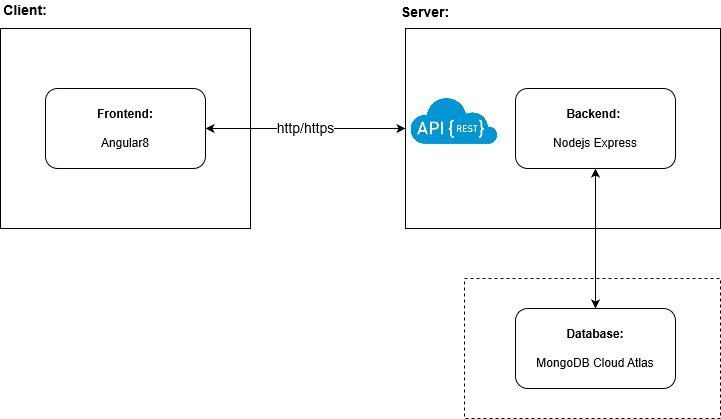
\includegraphics[width=0.8\textwidth]{architektur}
    \caption{Architektur Travelblog}
    \label{fig:architektur}
\end{figure}

\end{document}